\chapter{WLAN technologies and security}
With WLAN, as previously mentioned, we refer to a network that covers a small area. Actually, the most
common WLAN technology is Wi-Fi, which is based on IEEE 802.11 and trademarked.\\
Wifi supports mainly the infrastructure-based mode: which is usually made up of 
\begin{itemize}
  \item Access Points(APs)
  \item Wireless stations(STAs)
\end{itemize}
All the STAs are connected to the APs, which are connected to the wired network.\\
It actually supports ad-hoc mode, which uses direct communication, but it is not used that much.\\
  In infrastructure-based mode, all traffic must go through the AP, having no direct communication 
  possible. This is to solve the hidden terminal problem, where two STAs can't communicate because they
  can't hear each other, and 
\begin{figure}[h]
  \centering
  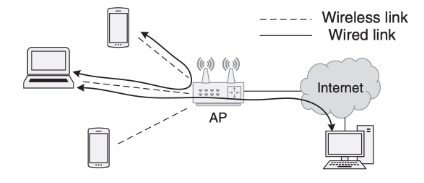
\includegraphics[width=0.7\textwidth]{img/wireless/wlan communication.png}
  \caption{Schema of a possible wireless communication}
\end{figure}
Furthermore, because it is based on 802.11, it carries over most of the standard:
\begin{itemize}
  \item \textbf{half-duplex communication channel}, at any time only one station can transmit or receive
  \item works on 2.4GHz and 5GHz bands, so multiplexing is available but quite limited
  \item uses \textbf{CSMA/CA} for medium access(carrier sense multiple access with collision avoidance)
\end{itemize}
The spectrum of the 2.4GHz band is divided into 14 channels, but only 3 of them are non-overlapping.
The 5GHz band has more channels, but it is less used because of the shorter range.
\begin{figure}
  \centering
  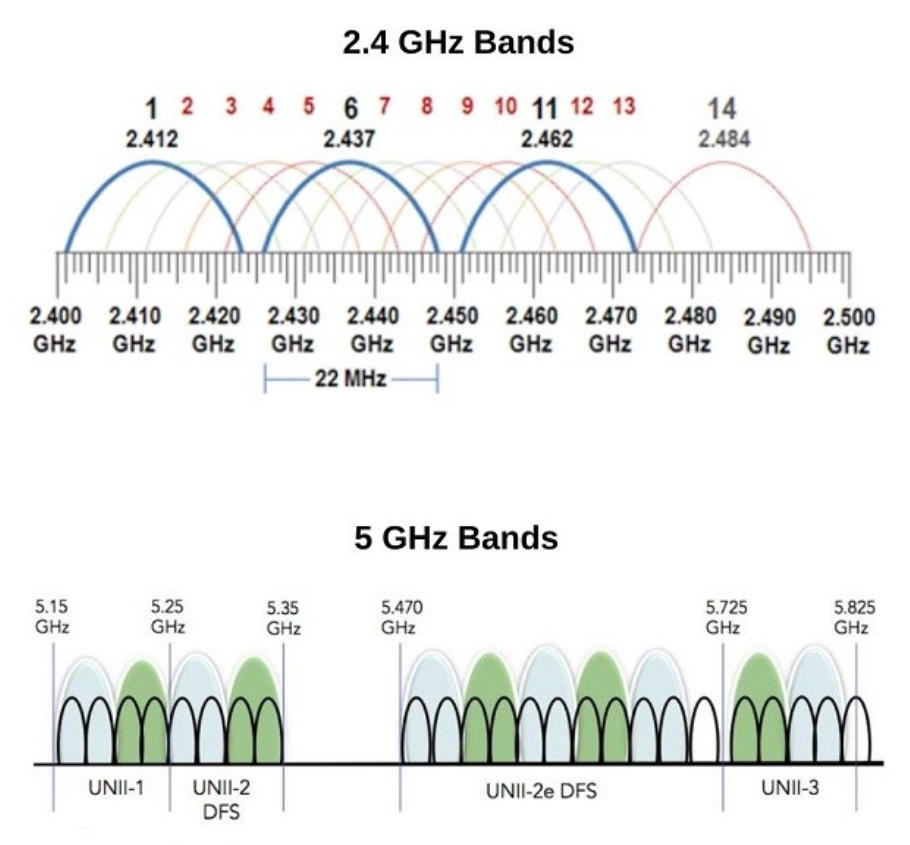
\includegraphics[width=0.5\textwidth]{img/wireless/80211 channels.png}
  \caption{802.11 channels}
\end{figure}
\begin{section}{WLAN Access}
  Before being able to access the network, an be able to send traffic trough an AP, a 
  mobile station can be:
  \begin{itemize}
    \item \textbf{Unauthenticated and unassociated}: the STA is not authenticated and not associated
    \item \textbf{Authenticated and unassociated}: the STA is authenticated but cannot transmit of receive 
      data
    \item \textbf{Authenticated and associated}: the STA is authenticated and associated
  \end{itemize}
  Data exchange is only possible in the last case.
  \begin{paragraph}{Authentication}
    \label{par:authentication}
    The 802.11 authentication is the first step to be performed. It requires the STA to prove its identity
    to the AP. During this step, no data encryption or security in general is provided.\\
    Usually the authentication is done with a shared key(WEP, WPA, WPA2, WP3), but it can also be 
    done with open system authentication, where the AP accepts any STA that wants to connect.\\
  \end{paragraph}
  \begin{paragraph}{Association}
    The 802.11 association is the second step to be performed. It requires the STA to select the AP to connect to,
    and to exchange information with it to gain access to the network.\\
    Association allows the AP to record each STA so that frames can be sent to the correct destination.
    Association only works in infrastructure mode, and a station can only be associated with one AP at a time.
    It is usually carried out as follows:
    \begin{itemize}
      \item After authentication, the STA sends an association request to the AP
      \item The AP processes the Association Request and decides if a client request should be allowed
        \subitem If the request is accepted it responds with a status code of 0 (successful) and the 
        Association ID (AID)
        \subitem Failed Association Requests include only a status code and the procedure ends
    \end{itemize}
  \end{paragraph}
  The STA must go through the following steps:
  \begin{enumerate}
    \item \textbf{Scanning(Beacon/probe)}: the STA scans the environment to find the APs
    \item \textbf{Association}: the STA selects the AP and sends an association request
    \item \textbf{Authentication}: the AP sends an authentication request to the STA
    \item \textbf{Authentication}: the STA sends an authentication response to the AP
    \item \textbf{Association}: the AP sends an association response to the STA
    \item \textbf{Exchange of data}: the STA can now exchange data with the AP
  \end{enumerate}
  Authentication can be performed with multiple access points of the same network, but association can only
  be performed with one of them.
  \begin{figure}[h]
    \centering
    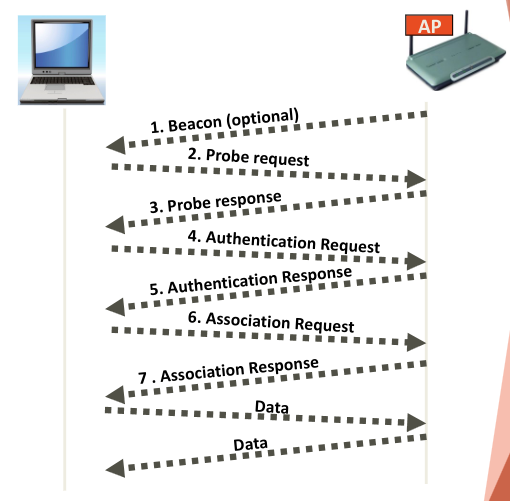
\includegraphics[width=0.5\textwidth]{img/wireless/wireless auth-ass.png}
    \caption{The authentication and association procedure in general}
  \end{figure}
  \begin{subsection}{Scanning for Access Points}
    To access the network, the mobile station must first associate with an access point.\\
    The \textbf{scanning process} is used to find the APs in the area, and it can be:
    \begin{itemize}
      \item \textbf{Passive scanning}: the STA listens to the beacon frames sent by the APs
      \item \textbf{Active scanning}: the STA sends a probe request to the APs in the area,
        and the APs respond with a probe response.
    \end{itemize}
    The beacon frames contains the informations needed to connect to the AP, such as the SSID, the
    mac address, the supported data rates, \dots, and every access point sends a beacon frame periodically, 
    usually every 100ms, as requested by the standard, even tough it can be disabled.\\
    Those informations are also contained in the probe response, which is sent by the AP in response to the
    probe request.
    \begin{figure}[h]
      \centering
      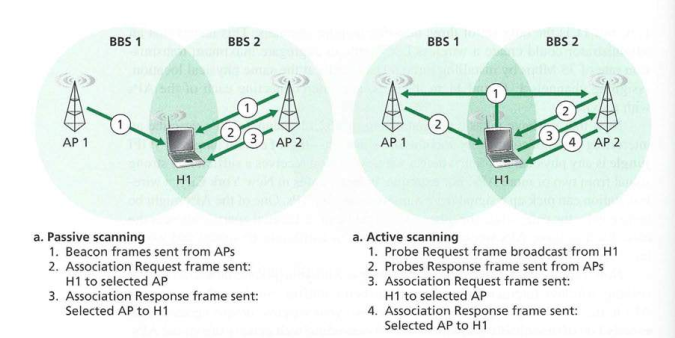
\includegraphics[width=0.8\textwidth]{img/wireless/wlan scanning.png}
      \caption{The two scanning methods}
    \end{figure}
  \end{subsection}
\end{section}
\begin{section}{Problems with 802.11}
  As already said in the chapter about wireless, the medium is unrealibale and the channel is shared, so
  there are some problems that have to be addressed.
  \begin{subsection}{Hidden terminal problem}
    The hidden terminal problem is a problem that arises when two stations can't hear each other, but they
    can hear the same access point.\\
    This can happen, for example, when two stations are too far from each other, but they are close 
    to the AP, or there's an obstacle between them.\\
    This problem is illustrated in figure \ref{fig:hidden terminal problem}.
    Issues can arise in this scenario: because the stations cant hear each other, they are unaware
    of the interntions of the other, so they are able to transmit at the same time, generating
    conflicts over the channel.
    \begin{figure}[h]
      \centering
      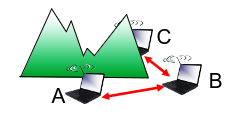
\includegraphics[width=0.5\textwidth]{img/wireless/hidden terminal problem.png}
      \caption{Hidden terminal problem}
      \label{fig:hidden terminal problem}
    \end{figure}
    Suppose that Station A is transmitting to Station B, which is also receiving from Station C.\\
    Station C can't hear Station A, so it will transmit, causing a collision at Station B.
  \end{subsection}
  \begin{subsection}{Fading}
    A second scenario that results in undetectable collisions at the receiver is fading.\\
    With fading we refer to the fact that the signal loses strength as it propagates through the medium.\\
    Figure \ref{fig:fading} shows the fading problem. A and C are placed such that their signals 
    are not strong enough to detect each other's transmissions , yet their signals are strong 
    enough to interfere with each other at station B.
    \begin{figure}[h]
      \centering
      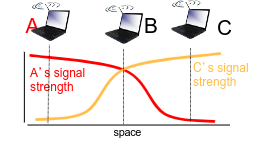
\includegraphics[width=0.5\textwidth]{img/wireless/fading.png}
      \caption{Fading}
      \label{fig:fading}
    \end{figure}
  \end{subsection}
  As previously said, 802.11 uses a half-duplex channel, so only one station can transmit at a time.
  \begin{subsection}{CSMA/CA}
    \label{sub:CSMA/CA}
    Since the channel is shared, the 802.11 standard uses CSMA/CA to avoid collisions, which is a 
    random access protocol similar to the CSMA/CD used in Ethernet.\\
    It implements collision avoidance instead of detection for two reasons:
    \begin{itemize}
      \item I requires a full duplex channel, and because the signals are very weak, it can be very
        costly to implement
      \item fading and hidden terminal problems make it difficult to detect collisions
    \end{itemize}
    For those reasons, once a station begins to transmit a frame, it transmits the frame in its 
    entirety, which, if you think about it, would increase the probability of a collision, degrading
    the performance of the network.\\
    Keep also in mind that 802.11 uses link-layer acknowledgements, so if an acknowledgement is not
    received after a certain time, it is retransmitted, and after a certain number of retransmissions,
    the frame is dropped.
    The CSMA/CA protocol is as follows: suppose that a station wants to transmit a frame
    \begin{enumerate}
      \item If initially the station senses the channel idle, it transmits its frame after a short 
        period of time known as the Distributed Inter-frame Space (DIFS)
      \item Otherwise, the station chooses a random backoff value using binary exponential backoff 
         and counts down this value after DIFS when the channel is sensed idle. While the channel 
         is sensed busy, the counter value remains frozen.
      \item When the counter reaches zero (note that this can only occur while the channel is 
        sensed idle), the station transmits the entire frame and then waits for an acknowledgment.
      \item If an acknowledgment is received, the transmitting station knows that its frame has 
        been correctly received at the destination station. If the station has another 
        frame to send, it begins the CSMA/CA protocol at step 2. If the acknowledgment isn't 
        received, the transmitting station reenters the backoff phase in step 2, with the random 
        value chosen from a larger interval.
    \end{enumerate}
    The goal is thus avoiding collisions whenever possible, hoping that by choosing a random
    backoff value, the stations will not choose the same value, and thus will not transmit at the
    same time.
    \begin{subsubsection}{RTS and CTS}
      802.11 also includes a optional reservation scheme, which is used to reserve the channel before
      transmitting a frame.\\
      The station that wants to transmit a frame can send a short \textbf{Request to Send(RTS)} 
      control frame and a short \textbf{Clear to Send(CTS)} control frame to \textit{reserve} the
      access to the channel.\\
      When a sender wants to send a DATA frame, it can first send an RTS frame to the AP, indicating 
      the total time required to transmit the DATA frame and the acknowledgment (ACK) frame. When 
      the AP receives the RTS frame , it responds by broadcasting a CTS frame. This CTS frame serves 
      two purposes: It gives the sender explicit permission to send and also instructs the other 
      stations not to send for the reserved duration.\\
      This technique make other station refrain from sending, thus reducing the probability of
      collisions, and solving the hidden terminal problem, at the cost of a higher overhead.
      \begin{figure}[h]
        \centering
        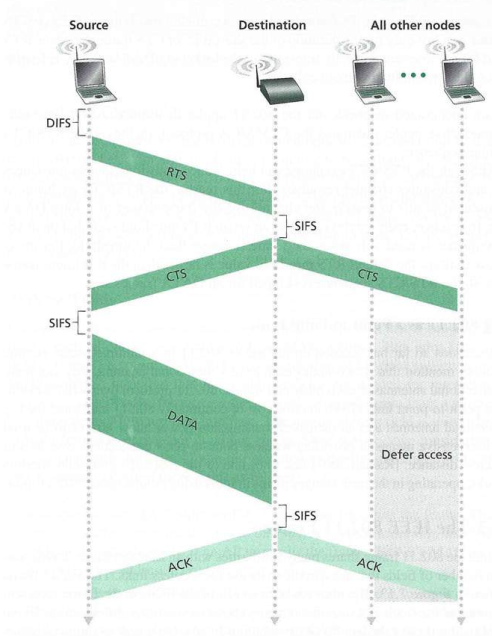
\includegraphics[width=0.5\textwidth]{img/wireless/cmsa with RTS.png}
        \caption{Collision avoidance with RTS/CTS}
        \label{fig:rts-cts}
      \end{figure}

    \end{subsubsection}

  \end{subsection}
\end{section}
\begin{section}{802.11 Features}
  \begin{subsection}{Frame Addressing}
    Although the 802.11 frame shares many similarities with an Ethernet frame, it also contains a 
    number of fields that are specific to its use for wireless links.\\
    The frame format is shown in figure \ref{fig:80211 frame format}.
    \begin{figure}[h]
      \centering
      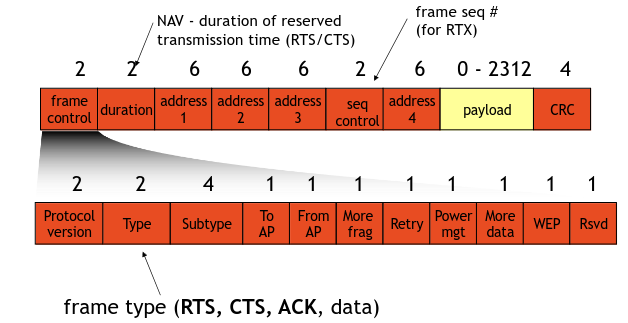
\includegraphics[width=0.5\textwidth]{img/wireless/802.11 frame.png.png}
      \caption{802.11 frame format}
      \label{fig:80211 frame format}
    \end{figure}
  \end{subsection}
  The numbers above each of the fields in the frame represent the lengths of the fields in bytes.
  The duration field is used to indicate the amount of time required to transmit the frame, and is 
  used for power saving.\\
  After that there are 4 address fields:
  \begin{itemize}
    \item The \textbf{address 1} is the MAC address of the station that is to receive the frame.
    \item The \textbf{address 2} is the MAC address of the station that is transmitting 
      the frame.
    \item The \textbf{address 3} contains the MAC address of the router interface of the subnet.
    \item The \textbf{address 4} is used in ad-hoc mode, and is the MAC address of the 
      destination station.
  \end{itemize}
  \begin{subsection}{Rate adaptation}
    802.11 also supports rate adaptation, which is the ability to change the transmission rate 
    based on the quality of the channel.\\
    This is necessary because the channel conditions can change rapidly, especially with mobile
    stations. In fact, As node moves away from base station, SNR decreases, BER(Bit Error Rate) increases
    If the modulation technique used in the 802.11 protocol operating between the base
    station and the user does not change, the BER will become unacceptably high as the
    SNR decreases, and eventually no transmitted frames will be received correctly.
    Base station and mobile dynamically change transmission rate (physical layer modulation technique) 
    as the mobile station moves, and the SNR varies as a result.
  \end{subsection}
  \begin{subsection}{Power Management}
    \label{sub:power management}
    Power is a precious resource in mobile devices, and thus the 802.11 standard provides 
    power-management capabilities that allow 802.11 nodes to minimize the amount of time that 
    their sense, transmit, and receive functions and other circuitry need to be "on".\\
    A node is able to explicitly alternate between asleep and awake states. A node signals to the 
    access point that it will be going to sleep by setting the power-management bit in the header 
    of an frame. A timer in the node is then set to wake up the node just before the AP is 
    scheduled to send its beacon frame.\\
    Since the AP knows from the set power-transmission bit that the node is going to sleep, it wont
    send any, and will buffer any frames destined for the sleeping host for later transmission.\\ A
    node will wake up just before the AP sends a beacon frame, and quickly enter the fully active
    state.
    The beacon frames sent out by the AP contain a list of nodes whose frames have been buffered 
    at the AP. If there are no buffered frames for the node, it can go back to sleep. Otherwise, 
    the node can explicitly request that the buffered frames be sent by sending a polling message 
    to the AP.

    \begin{figure}[h]
      \centering
      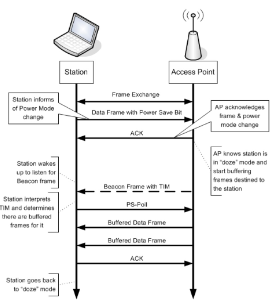
\includegraphics[width=0.5\textwidth]{img/wireless/80211 power saving.png}
      \caption{Power management in 802.11}
    \end{figure}

  \end{subsection}

\end{section}
\begin{section}{Performance evaluation of 802.11}
  As seen in the previous sections, 802.11 has some features that can be used to improve the
  performance of the network, and is also divided into different version with different 
  throughput: 802.11b(up to 11Mbps), 802.11a(up to 54Mbps), 802.11g(up to 54Mbps), 802.11n(up to 600Mbps),
  \dots\\
  Event tough the throughput is high, the actual goodput is much lower, because of the overhead
  introduced by the protocol, the hidden terminal problem, the collision avoidance, and the fading.\\
  The goodput can be defined as the speed at which useful data is received at the application layer,
  Given the capacity C at the physical layer, and can be calculated as follows:
  \begin{equation}
    G = \frac{\text{(Useful data at the application layer)}}{\text{(time to complete the tranfer)}<C}
  \end{equation}
  which will of course be lower than the capacity C.\\
  Given this definition, we can observe that the goodput is reduced by each layer of the protocol stack,
  because each of them adds control information that is useful to provide the service but is not part of
  the useful data, and that the actual goodput is much lower than the theoretical throughput.\\
  \begin{figure}[h]
    \centering
    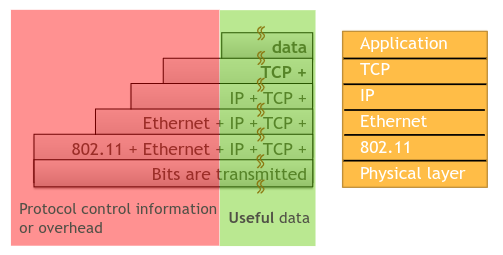
\includegraphics[width=0.5\textwidth]{img/wireless/encapsulation overhead.png}
    \caption{The overhead that each packet has to carry}
  \end{figure}
  Furthermore, several factors can reduce the goodput, for example:
  \begin{itemize}
    \item shared physical link with other protocols and transmissions
    \item errors: bit error, congestion, packets drops, you name it
    \item retransmissions: if a packet is lost, it has to be retransmitted
    \item \dots 
  \end{itemize}
  This means that the actual goodput is always less than the protocol efficiency, which is the
  ratio between the useful data and the total data sent per the capacity of the channel.\\

  
  \begin{table}[h]
    \centering
    \begin{tabular}{|c|c|}
      \hline
      Protocol & Overhead \\
      \hline
      TCP & 20 bytes per segment\\
      \hline
      UDP & 8 bytes\\
      \hline
      IP & 20 bytes\\
      \hline
      Ethernet & 38 bytes(8 (trailer + SoF) + 6 (MAC) + 6(MAC) + 2 (Type) + 4 (CRC) + 12 (IPG))\\
      \hline
    \end{tabular}
    \caption{Overhead introduced at each layer per packet}
  \end{table}
  % tabular 2 columns: protocol|overhead
  \begin{subsubsection}{Efficiency of TCP/IPv4/Ethernet}
    The efficiency of the TCP/IP/Ethernet stack can be calculated as follows: we know that the 
    maximum MTU for ethernet is 1500 bytes, and that the maximum payload for an IP packet is 1500-20=1480
    bytes, and that the maximum payload for a TCP segment is 1480-20=1460 bytes.\\
    This overhead is applied to each segment, and because its more likely that the payload at application 
    level is larger than the TCP MTU, there will probably be more segments.\\
    So the efficiency of the TCP/IP/Ethernet stack is:
    \begin{equation}
      \eta_{TCP} = \frac{\text{L7 data}}{\text{Transmitted data}} = \frac{1460}{1460+20+20+38} = 94\%
    \end{equation}
    This was in case the channel if full-duplex, but if it is half-duplex, the efficiency is reduced, because
    the ack packets have to be sent in the opposite direction, and the channel can't be used to send data
    in that direction.\\
    The efficiency of the TCP/IP/Ethernet stack in half-duplex is:
    \begin{equation}
      \eta_{TCP} = \frac{\text{L7 data}}{\text{Transmitted data}} = \frac{1460}{(1460+20+20+38)+(20+20+38)} = 90\%
    \end{equation}
    In general, To calculate the total efficiency, it is sufficient to make the product of the
    individual efficiencies.
  \end{subsubsection}
  \begin{subsection}{Theoretical Maximum Throughput}
    The theoretical maximum throughput is a difficult value to calculate, because different parts 
    of the frame are transmitted at different rate: for example, the header is transmitted at a 
    lower rate than the payload(1Mbps).\\
    As such, the theoretical maximum throughput of an application which uses 802.11 is calculated as follows:
    \begin{equation}
      TMT_{APP} = \frac{\beta}{\alpha + \beta}\times TMT_{802.11}(\text{bps})
    \end{equation}
    where $\alpha$ is the total overhead above the MAC layer, and $\beta$ is the application layer
    datagram size.\\
    Computing $TMT_{802.11}$ is a bit more difficult, because some components of the protocol are variable
    but we can approximate it when the scenario is ideal:
    \begin{itemize}
      \item the bit to error rate is 0
      \item there are no losses due to collisions
      \item no packet is lost at the receiving node
      \item PCF mode is not used 
      \item the sending node always has a sufficient number of packets to send
      \item no fragmentation is used at level 2
    \end{itemize}
    but in general we need to consider the ratio between the time in which useful data is sent 
    and the one needed for the overhead.\\
    We can thus consider the TMT as:
    \begin{equation}
      TMT = \frac{\text{MSDU size}}{\text{Delay per MSDU}}
    \end{equation}
    where MSDU is MAC service data unit, which carries the actual data that needs to be transmitted,
    and the delay per MSDU is the time needed to transmit the MSDU, which is overhead time + data time:
    \begin{equation}
      \text{Delay per MSDU} = (T_{DIFS} + T_{SIFS} + T_{BO} + T_{RTS} + T_{CTS} + T_{ACK} + T_{DATA}) \times 10^{-6}s
    \end{equation}
    All those values varies on the mode used:
    \begin{figure}[H]
      \centering
      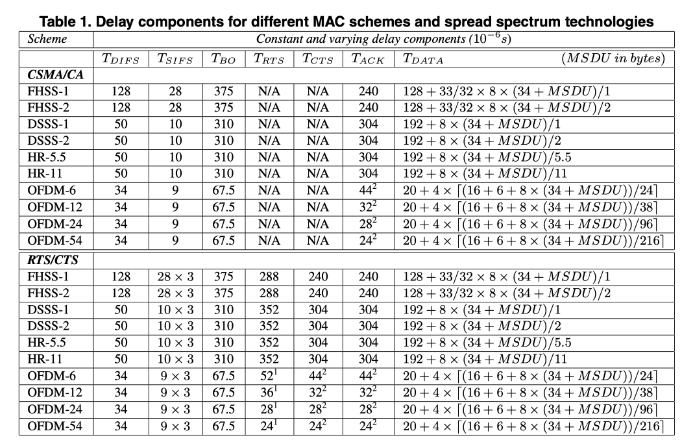
\includegraphics[width=0.7\textwidth]{img/wireless/delay components.png}
    \end{figure}
  \end{subsection}
\end{section}
\begin{section}{Security issues of WLAN}
  More and more security issues arise when using a wireless medium, and this is also true when using
  802.11.
  \begin{subsection}{Denial of Service}
    Denial of Service is a quite common attack at layer 2, and also quite old, since it has been demonstrated in
    2003, and it is still possible today.
    \begin{boxH}
      Denial of Service is a type of attack that aims to make a network service unavailable to 
      a user, by overwhelming the client with more traffic that it can handle.
    \end{boxH}
    In fact, 802.11 is "more vulnerable" than ethernet, because it is a shared medium, and the attacker
    can easily listen and transmit any frame.\\
    A dos attack can be performed either:
    \begin{itemize}
      \item \textbf{at the physical layer}: by sending a jamming signal, the attacker can prevent the 
        receiver from receiving the frame
      \item \textbf{at the MAC layer}: which mostly rely on the identification problems of 802.11
    \end{itemize}
    With identification problems we refer to the fact that nodes are identified by their MAC address,
    which can be easily spoofed, because there's no authentication at the MAC layer.\\
    Based on this simple fact, there are several attacks that can be performed.
    \begin{subsubsection}{Disassociation attack}
      Before going over this kind of attack, a quick reminder that a client can authenticate with
      multiple APs, but can only be associated with one of them.\\
      There's also another kind of frame, the disassociation frame, which is used to terminate the
      connection between a client and an AP, which is not authenticated, like the association one.\\
      This meas that an attack can, at any point of the connection, send a disassociation frame to the
      AP while spoofing the MAC address of the client, and the AP will terminate the connection with the
      client.\\
      By repeating this process, the attacker can prevent the client from connecting to the network, and
      thus from receiving any data, performing a denial of service attack.
      \begin{figure}[h]
        \centering
        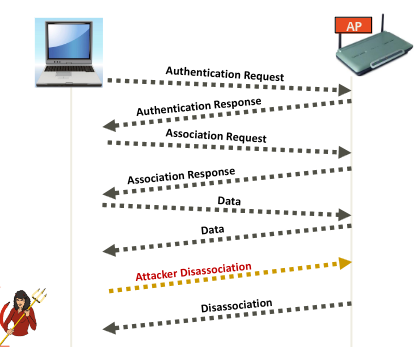
\includegraphics[width=0.6\textwidth]{img/wireless/disassociation attack.png}
        \caption{Example of a disassociation attack}
      \end{figure}

    \end{subsubsection}
    \begin{subsubsection}{Deauthentication attack}
      The general principle of 802.11 authentication has already been explained in paragraph
      \ref{par:authentication}, but it is worth mentioning that the deauthentication frame is used to
      terminate the authentication process.\\
      As such, it is possible to perform a deauthentication attack, in the same fashion as the
      disassociation attack, by sending a deauthentication frame to the AP while spoofing the MAC address
      of the client.\\
      Doing so, the client must re-authenticate with the AP, and if the attack is repeated, the client
      will be unable to connect to the network, and thus to receive any data, performing a denial of
      service attack.\\
      This kind of attack can be executed on individual clients, or on the whole network, by spoofing
      the AP address, and sending the deauthentication frame to all the clients.

      \begin{figure}[h]
        \centering
        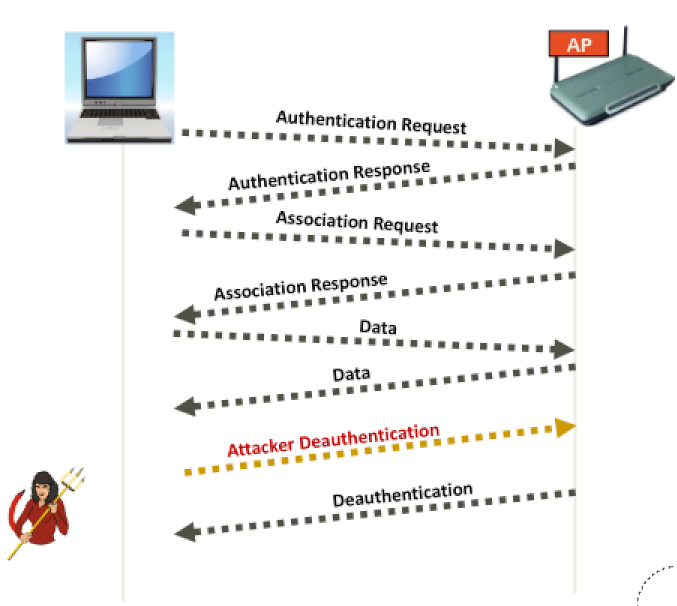
\includegraphics[width=0.6\textwidth]{img/wireless/deauthentication attack.png}
        \caption{Example of a deauthentication attack}
      \end{figure}

    \end{subsubsection}
    \begin{subsubsection}{Protection against deauthentication attacks}
      In general, it is better to implement a protection against deauthentication attacks, because 
      after a deauthentication attack, the client will need 2RTTs to resume the communication,
      while after a disassociation attack, the client will need only 1RTT.\\
      A simple protection against deauthentication attacks that as been proposed is based on the 
      observation that legitimate nodes do not deauthenticate themselves and then send data.
      As such, an AP can delay the honoring of a deauthentication frame for a short period of time,
      and if any frames are sent by the client, the deauthentication frame is ignored.\\
      This solution is quite good because it requires no modification to the protocol and its 
      backward compatible.\\
      Another solution is to use the SNR of the signal as a "signature" of the client, and if the
      SNR doesn't match the signature, the deauthentication frame is ignored.
    \end{subsubsection}
    \begin{subsubsection}{Attacks on CSMA-CD}
      The general principle of CSMA-CD has already been explained in paragraph \ref{sub:CSMA/CA},
      but it is worth mentioning that it is possible to perform a denial of service attack by
      sending a signal before every SIFS slot, which will prevent the other nodes from transmitting
      the frame, because they will sense the channel as busy.\\
      So just by sending 50000 frames per second, which is roughly one tenth of the capacity of the
      channel, the attacker can shut down the channel.\\
      The attack that has been just explained only works if RTS/CTS is not used, but its also possible
      to perform an attack even in the opposite case. In fact, in a RTS request it is possible to 
      specify the reservation time, with a 2 byte field, and by setting it to a large value,
      the attacker can prevent the other nodes from transmitting. 
      \begin{figure}[h]
        \centering
        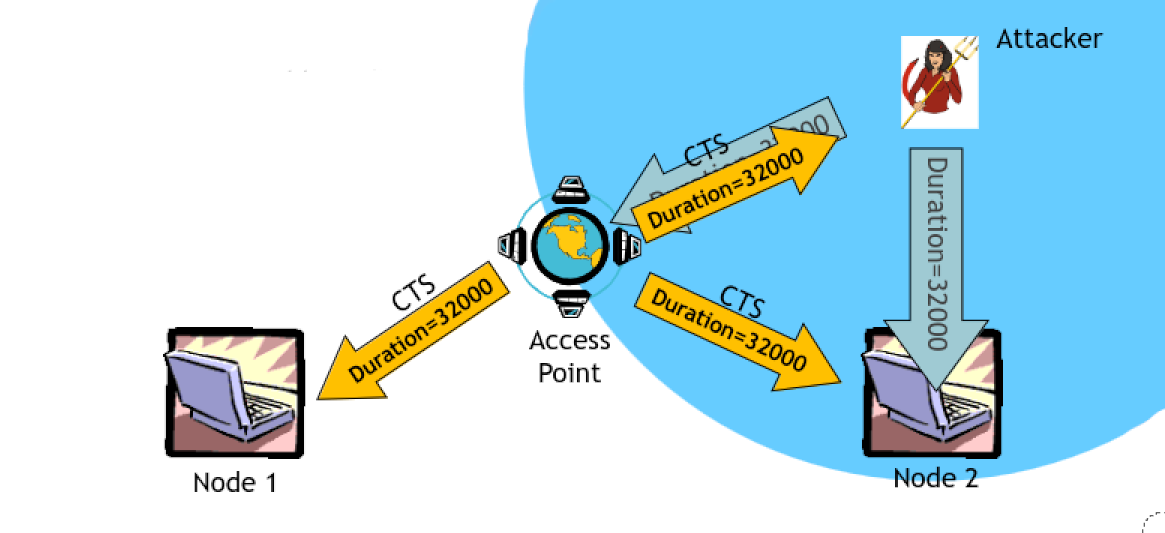
\includegraphics[width=0.6\textwidth]{img/wireless/RTS attack.png}
        \caption{Example of a CSMA-CD/RTS attack, the attacker sets a large value in the RTS request}
      \end{figure}
      To prevent this kind of attack it is possible to set a reasonable limit on the reservation time,
      because all legitimate traffic use relatively small values. 
    \end{subsubsection}
    \begin{subsubsection}{Attack on power saving}
      As seen in in subsection \ref{sub:power management}, 802.11 has a power saving mode, which allows
      the client to go to sleep, and wake up only when it is needed.\\
      To signal that a station is going to sleep, it sends a Null data frame with the power management
      bit set.\\
      Multiple attacks can be performed on this mechanism:
      \begin{itemize}
        \item An attacker can spoof on behalf of AP the TIM message, which is used to signal the clients
          that there are packets waiting for them, making the clients think that there are no packets
          waiting for them, and thus go to sleep
        \item An attacker forge management sync packets, causing them to fall out of sync with the AP
        \item An attacker spoof on behalf of the client, making the AP send data while the client is 
          sleeping
      \end{itemize}
      Let's now describe the latter scenario: of course an attacker can impersonate the victim STA,
      because he just needs to know the MAC addresses of the AP and the victim. The attacker can 
      keep injecting \textbf{false power management frames} to the AP, which will make the AP think
      that the victim is going to sleep, and thus it will buffer the packets.\\
      The AP sends a Beacon frame with the TIM (Traffic Indication Map) to signal the victim to 
      wake-up, but the victim will ignore those, because it's not in power management mode.\\
      \begin{figure}[h]
        \centering
        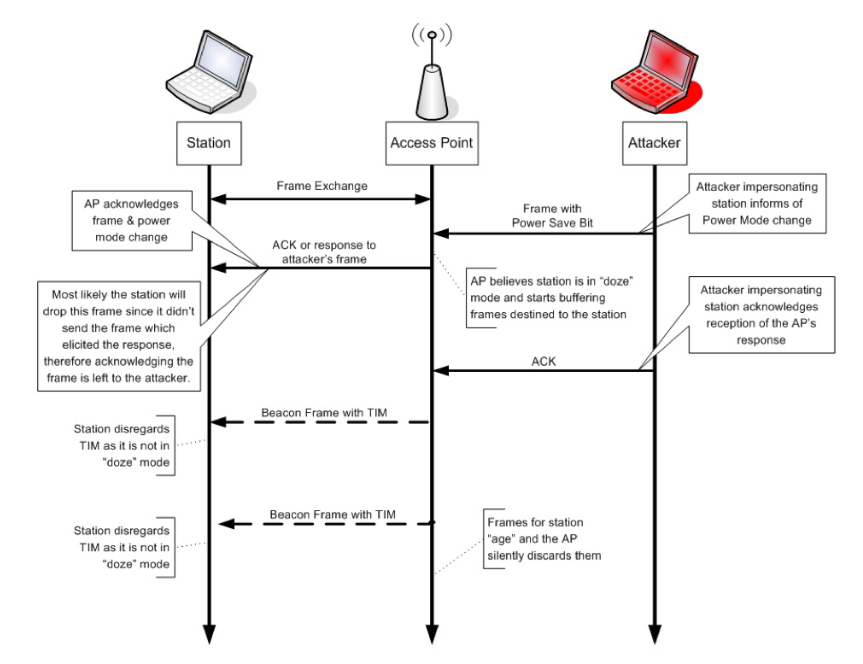
\includegraphics[width=0.7\textwidth]{img/wireless/power saving attack.png}
        \caption{Example of a power saving attack}
      \end{figure}

    \end{subsubsection}

  \end{subsection}
  Although all those issues were published in 2003, the threats are still present today, making DoS 
  an deauthentication attacks still possible today.

\end{section}
\begin{section}{WLAN security}
    As per the previous section, we also learned that:
    \begin{itemize}
      \item MAC authentication is useless, because is sent in broadcast, so can be sniffed and replayed
      \item static IP addresses are useless, because can be easily sniffed from the packets
      \item SSID hiding is useless, because even if we can suppress beacons frames, SSID are sent 
        in clear text in probe request/response and association response
      \item Smart antenna placement and hiding is useless, because the attacker can have more resources 
        and this also impact the final users
    \end{itemize}
    The only real solution is to use encryption, and a secure standard while we are at it.
  \begin{subsection}{WEP}
    \begin{boxH}
      WEP stands for Wired Equivalent Privacy, and is a security protocol used in wireless networks.
    \end{boxH}
    It was first introduced in 1998, so it's a quite old standard, and was intended to protect 
    wireless confidentiality comparable with that of a traditional wired network and intended to 
    achieve the following security goals:
    \begin{itemize}
      \item \textbf{Confidentiality} via encryption 
      \item \textbf{Access control} via shared password authentication
      \item \textbf{Data integrity} via checksums
    \end{itemize}
    Actually WEP was never meant to achieve strong security, but it's better than nothing, even if 
    it has some serious flaws, which make it fail to achieve the security goals, or properties, 
    which were:
    \begin{itemize}
      \item To be reasonably strong, by changing frequently the \textit{IV}, and hence the key $k$,
        to avoid statistical attacks, which are possible with a fixed key
      \item To be self-synchronizing, otherwise it would be difficult to decrypt the messages.
        This property is provided by the IV itself, as using a reliable data transmission protocol
        would hinder the performance too much.
      \item To be efficient, by using a stream cipher
      \item To be IP(Intellectual property) free
      \item To be exportable, which is a requirement for the US government
    \end{itemize}
    \begin{subsubsection}{WEP access control}
      WEP implements two different authentication methods:
      \begin{itemize}
        \item \textbf{Open system authentication}: which is the default one, and is used when the 
          client wants to connect to the network
        \item \textbf{Shared key authentication}: which is used when the client wants to connect to the 
          network, and is based on a shared key
      \end{itemize}
      The shared key authentication is based on a challenge-response mechanism, where the AP sends a
      challenge to the client, which has to respond with the correct response, which is based on the
      shared key.\\
      Once authenticated, the STA can send an association request and the AP will respond with an 
      association response. If authentication fails, no association is possible.
      The challenge is based on the RC4 algorithm, which is a stream cipher which is known to be not 
      the most secure nowadays, but at the time was considered secure enough.\\
      \begin{figure}[h]
        \centering
        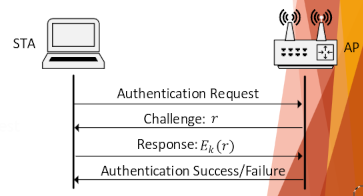
\includegraphics[width=0.5\textwidth]{img/wireless/WEP authentication.png}
        \caption{The CRA authentication scheme of WEP}
      \end{figure}
      Counter intuitively, the shared key authentication is less secure than the open system
      authentication, because a bruteforce attack can be mounted on the challenge frame, because both 
      the cyphertext(it's 128 bits long) and the algorithm(RC4) are known.\\
      Thus, data can be more easily intercepted and decrypted with Shared Key authentication than 
      with Open System authentication
      If privacy is a primary concern, it is more advisable to use Open System authentication for WEP
      authentication, but this schema doesn't allow WLAN clients to connect to the AP.

      \begin{figure}[h]
        \centering
        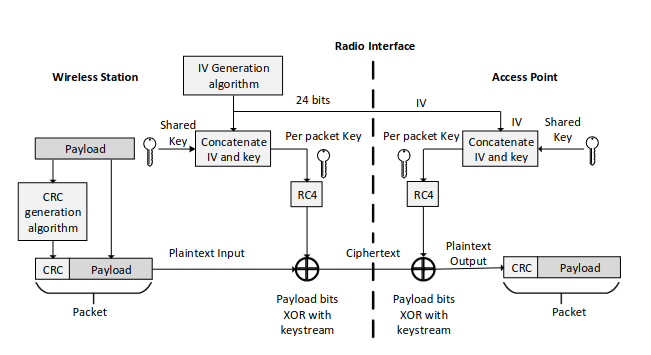
\includegraphics[width=0.5\textwidth]{img/wireless/WEP security.png}
        \caption{General overview of WEP security}
      \end{figure}
    \end{subsubsection}
    \begin{subsubsection}{WEP integrity and confidentiality}
      As for what concerns the integrity of the data, WEP uses a checksum, which is a CRC32(Cyclic
      Redundancy Check) checksum of 32 bits, which is appended to the frame.
      RC4 is initialized with the shared key between the STA and the AP and the IV, and for each 
      message to be sent: 
      \begin{itemize}
        \item RC4 produces a pseudo-random sequence of bits
        \item The sequence is XORed with the message
      \end{itemize}
      The reception is carried out in the same way. To guarantee the confidentiality of the message,
      each frame have to be encrypted with a different key stream, using the RC4 algorithm.
    \end{subsubsection}
    \begin{subsubsection}{WEP Key Management}
      Two kind of keys are used in WEP:
      \begin{itemize}
        \item \textbf{Default key}, also called \textit{shared key}
        \item \textbf{Key mapping keys}, also called \textit{individual keys}
      \end{itemize}
      but in practice, only the default key is used, because the key mapping keys are not used in the
      standard. This has some serious implication, because the cey between the AP and all the STA 
      is the same, each STA can decrypt the frames sent by another STA.\\
      Furthermore, the default key has to be changed if a member leaves the group, to make it impossible
      for it to get back in the network by itself, but this is quite impractical, because the 
      key has to be changed on every device simultaneously, which is quite difficult.\\
      For those reasons, WEP supports multiple default keys, with only the "active key" used for encryption, 
      and any of the keys can be used for decryption.\\
      The message header contains a key ID that allows the receiver to find out which key should be used
      to decrypt the message.

      \begin{figure}[h]
        \centering
        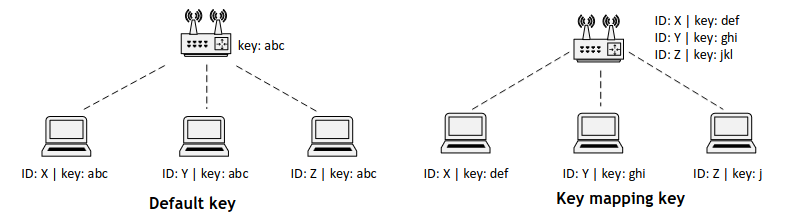
\includegraphics[width=0.5\textwidth]{img/wireless/WEP key management.png}
        \caption{WEP key management}
      \end{figure}

    \end{subsubsection}
    \begin{subsubsection}{Issues with authentication and access control}
      As previously said, WEP authentication is based on challenge-response using RC4. Knowing that
      the response is $E_k(r)=r\oplus L$, where $r$ is the challenge, an attacker that is listening 
      to the conversation can easily recover the key $k$ by XORing the challenge with the response(
      $K=r\oplus E_k(r)$). WEP doesn't provide AP authentication, so it's very easy for an attacker
      to impersonate the AP, even if they don't know the key, by just broadcasting the same SSID as the
      AP, but with an higher signal strength. It's also possible to do this for all the SSIDs(karma attack).
    \end{subsubsection}
    \begin{subsubsection}{Issues with integrity and replay}
      First of all, WEP doesn't provide any protection against replay attacks, because the IV is
      not changed after each message.\\
      Furthermore, if a CRC-32 valid plaintext is XORed with a ciphertext, the modified message 
      will pass the ICV check after decryption. In fact an attacker can observe $C=(M|CRC(M))\oplus K$
      where $K$ is the output of RC4.\\ 
      Then, for any $\Delta M'$ he can compute $CRC(\Delta M)$:
      \begin{equation}
        \begin{split}
        &((M|CRC(M))\oplus K)\oplus (\Delta M|CRC(\Delta M)) =\\
        &((M\oplus \Delta M)|(CRC(M)\oplus CRC(\Delta M)))\oplus K=\\
        &((M\oplus \Delta M)|(CRC(M)\oplus CRC(\Delta M)))\oplus K
        \end{split}
      \end{equation}
      Doing so, an attacker can arbitrarily modify the message, and the receiver will not be able to
      detect it.
    \end{subsubsection}
    \begin{subsubsection}{Issues with confidentiality}
      The ICR can be also attacked to retreive the content of the original message. In fact, if an
      AP receives a packet that does not pass the ICV check, it will not be accepted and sent in the network,
      so an attacker can create a corrupted packet, based on a captured one, and send it to the AP.
      By changing one byte at the time, the attacker can find the correct byte, and thus decrypt the
      message.\\
      Another issue that can arise is that the IV is only 24 bits long, so after $2^{24}$ packets,
      the same IV will be used again, and the key will be the same. An attacker can thus build a 
      \textit{decryption table} to perform a statistical attack.\\
      Furthermore, for some seed values (called weak key), the beginning of the RC4 output is
      not random: if a weak key is used, the first few bytes of the output reveals a lot of 
      information about the key, so breaking the key is a lot easier.
    \end{subsubsection}
  \end{subsection}
  
  \begin{subsection}{WPA}
    WEP is used only in the 802.11 vanilla, but is was soon replaced by 802.11 with the WPA(Wi-Fi
    protected access) standard. It was introduced to replace WEP, but it has some serious flaws:
    in fact, it dows not replace the chypher.\\
    Starting from 802.11i, the WPA2 standard was introduced, which is based on the AES encryption
    algorithm, which is much more secure than the RC4 used in WEP, and in 2018 the WPA3 standard
    was introduced, which is even more secure than WPA2.\\
    The main featured of the new standard were:
    \begin{itemize}
      \item improved integrity protection, by introducing Micheal 1 instead of CRC32
      \item improving the encryption algorithm, by using AES
      \item indroducing access control, by using 802.1x
    \end{itemize}
    but also had other killing features:
    \begin{itemize}
      \item flexible authentication framework (based on EAP – Extensible Authentication Protocol)
      \item authentication can be based on strong protocols (e.g., TLS – Transport Layer Security)
      \item authentication process results in a shared session key (which prevents session hijacking)
      \item different functions (encryption, integrity) use different keys derived from the session key using a
        one-way function
    \end{itemize}
    
    \begin{subsubsection}{802.1X authentication model}
      The authentication model of 802.1X is based on the following components:
      \begin{itemize}
        \item \textbf{Supplicant}: the client that wants to connect to the network
        \item \textbf{Authenticator}: the device that controls the access to the network. In most 
          cases, it is the AP
        \item \textbf{Authentication server}: the server that authenticates the client
      \end{itemize}
      A supplicant to get access to the network, has to authenticate itself to the authenticator 
      at first. If the authentication is successful, the authenticator server will instructs the authenticator 
      to let the device join the network, and thus access its services. The authentication server
      will then inform the supplicant that the access has been granted.\\
      \begin{figure}[h]
        \centering
        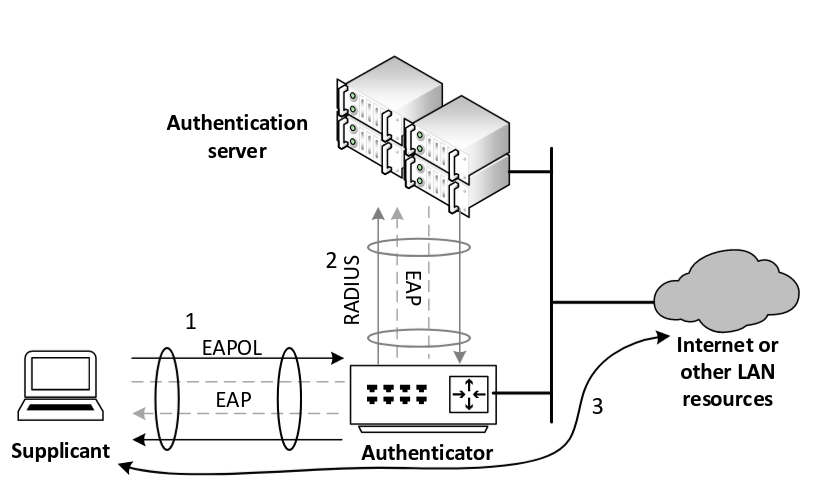
\includegraphics[width=0.5\textwidth]{img/wireless/WPA authentication.png}
        \caption{The general 802.1X authentication model}
      \end{figure}
      \begin{figure}[h]
        \centering
        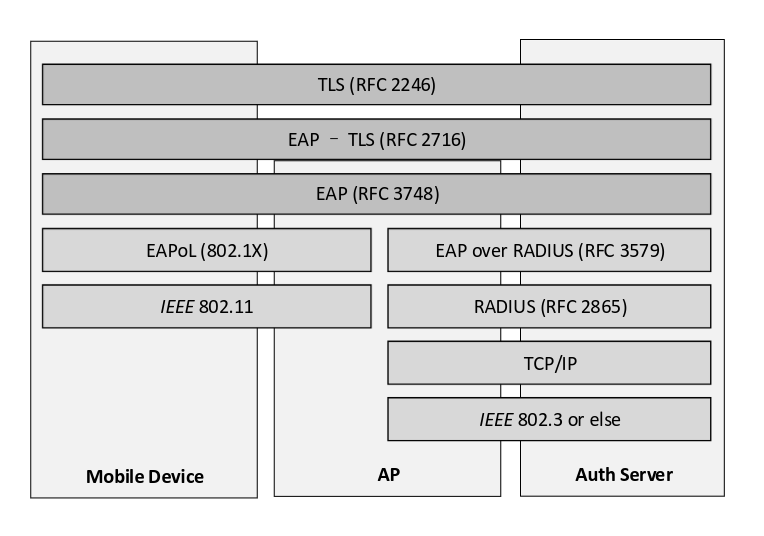
\includegraphics[width=0.5\textwidth]{img/wireless/802.1X protocol stack.png}
        \caption{The stack of protocols that can be used in 802.1X authentication}
      \end{figure}
      In 802.11i, after a successful authentication, the authenticator will generate a \textbf{session
      key} between the supplicant and the authentication server, which is sent to the AP in a secure 
      way. This assumes the use of a shared key between the AP and the authentication server, which is 
      usually set up by the network administrator.\\
    \end{subsubsection}
    The IEEE 802.11i standard defines two security protocols:
    \begin{itemize}
      \item \textbf{WPA}: Wi-Fi Protected Access, an optional protocol Temporal Key Integrity 
        Protocol (TKIP) to allow backward compatibility with WEP
      \item \textbf{WPA2}: Wi-Fi Protected Access 2, which uses the Advanced Encryption Standard 
        (AES) instead of RC4
    \end{itemize}
    \begin{subsubsection}{802.1X authentication protocols}
      802.1X authentication uses the EAP protocol, which is a carrier protocol that can be used with
      different authentication methods, like TLS, TTLS, PEAP, \dots. With this method, the
      authenticator only understands the outcome of the authentication, and not the messages itself.
      To transmitt its messages, EAP can use two protocols:
      \begin{itemize}
        \item \textbf{EAP over LAN(EAPOL)}: which is used to transmit the EAP messages over the 
          network by encapsulating them in Ethernet frames, and is used to carry EAP messages between
          the STA and the AP
        \item \textbf{RADIUS}: which is used to carry the EAP messages between the AP and the 
          authentication server
      \end{itemize}
      \begin{figure}[h]
        \centering
        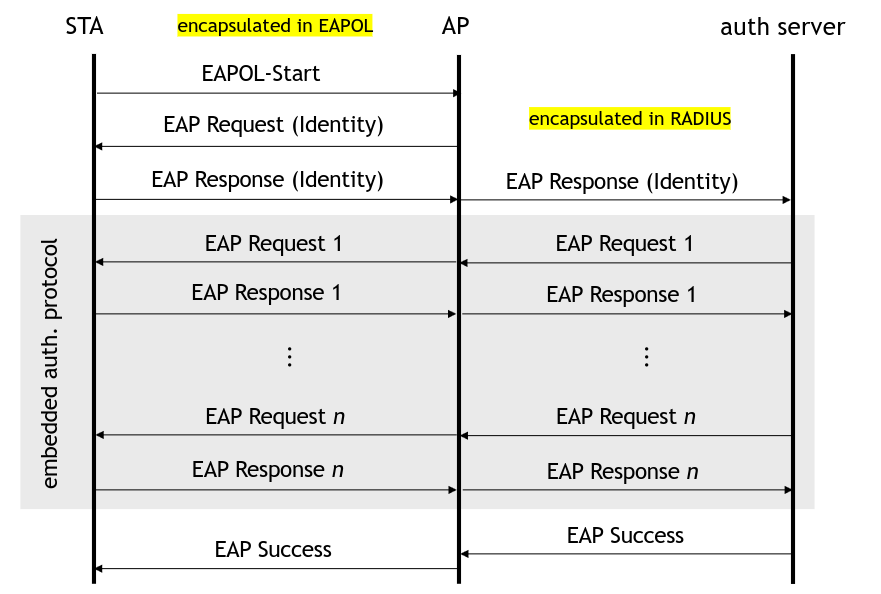
\includegraphics[width=0.5\textwidth]{img/wireless/EAP authentication.png}
        \caption{The general schema of the EAP authentication}
      \end{figure}
    \end{subsubsection}
    \begin{subsubsection}{802.11i Access Control}
      WPA supports two different kinds of authenticated key management protocols:
      \begin{itemize}
        \item \textbf{Pre-shared key(PSK)}: which is used in small networks, and is based on a 
          shared key between the AP and the STA. Its also called \textbf{WPA-Personal}
        \item \textbf{802.1X}: which is used in larger networks, and is based on a shared key between
          the AP and the authentication server, which requires a RADIUS server. It's also called
          \textbf{WPA-Enterprise}
      \end{itemize}
    \end{subsubsection}
    \begin{subsubsection}{Key management}
      A quick reminder that in WEP, all the STA share the same key, whcih generate some issues: in
      fact this application of confidentiality only protects the data from listeners outside from
      the network, but not inside. In WPA, this is not the case, because multiple keys are used,
      which are generated from the master key, \textbf{Pairwise Master Key(PMK)}, which
      is derived from the password, and is used to derive the PTK and the GTK.\\
      This PMK can be either:
      \begin{itemize}
        \item pre-shared in WPA-Personal
        \item derived from the EAP authentication in WPA-Enterprise
      \end{itemize}
      A different key between the AP and the STA is used, called the \textbf{Pairwise Transfer Key(PTK)},
      and derived from :
      \begin{itemize}
        \item the PMK
        \item the MAC addresses of the AP and the STA
        \item the nonce of the AP and the STA
      \end{itemize}
      The PTK is transient because every time a client associates with the AP, a new PTK is derived
      To allow confidentiality in broadcast communication, a \textbf{Group Transient Key(GTK)} is 
      used, which is shared between all the STA and the AP, computed by it and sent to all the STA.
      \begin{figure}[h]
        \centering
        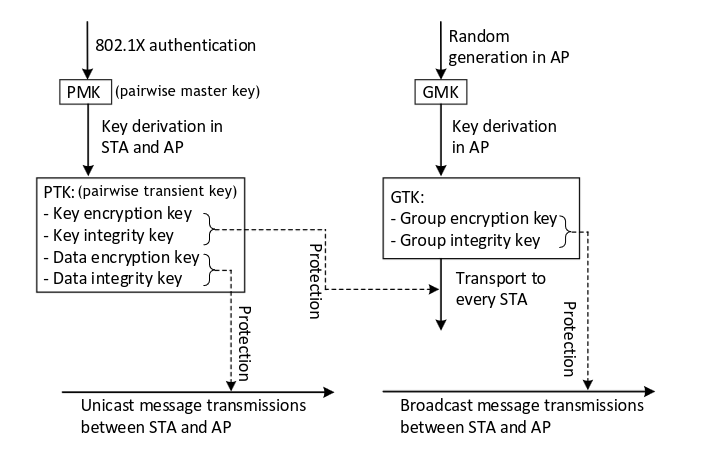
\includegraphics[width=0.7\textwidth]{img/wireless/WPA key hierarchy.png}
        \caption{Key hierarchy in WPA-802.1X}
      \end{figure}
    \end{subsubsection}
    \begin{subsubsection}{Four-way handshake}
      The four-way handshake is used to establish the PTK, and is used to authenticate the client
      to the AP, because it is based on the PMK, which is the result of the authentication.\\
      At first, the \textbf{AP sends} a \textbf{nonce} to the client in a \textbf{plaintext} message
      and without any integrity check.\\
      The \textbf{client} receives message and \textbf{derives} the
      $\text{PTK}=f(\text{PMK},\text{AP}_{\text{nonce}},\text{STA}_{\text{nonce}}
      ,\text{AP}_{\text{MAC}},\text{STA}_{\text{MAC}})$,
      and proceeds to send the second message, which contains the $\text{STA}_{\text{nonce}}$ and an integrity
      check, which is computed using \textbf{half} of the \textbf{PTK} to protect the message and
      \textbf{avoid brute force} attacks on the PTK. This message too is sent in plain.\\
      Once this message is received, the \textbf{AP computes} the \textbf{PTK} after having verified
      the integrity of the message, and sends the \textbf{third message}, which contains the
      \textbf{GTK} and its associated MIC(message integrity code), which is computed using the other
      half of the PTK. This message acts also as a request to install the key. After the client
      receives this message, it the MIC checks out, it means that the AP and the client have the
      same $PTK$, and the GTK is installed.\\
      One \textbf{last message} is sent by the client, which is an \textbf{acknowledgment} of the
      \textbf{GTK installation}, with its associated MIC. If the integrity check is successful, the
      AP installs the GTK and the PTK, and the client is authenticated, concluding the four-way
      handshake.

      \begin{figure}[h]
        \centering
        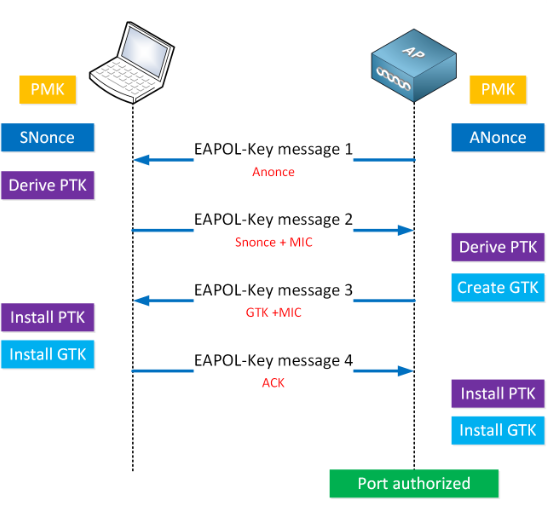
\includegraphics[width=0.5\textwidth]{img/wireless/4-way handshake.png}
        \caption{The four-way handshake in WPA using EAPOL}
      \end{figure}
    \end{subsubsection}
    \begin{subsubsection}{Bruteforce attack against WPA}
      During the 4-way handshake, a lot of informations are sent in clear: the key(not directly, but
      its there), the MAC addresses, the nonces, \dots\\
      An attacker can capture the challenge and the result, try all possible combinations offline to
      guess the key using a dictionary attack.\\
      This kind of attack is possible only if the key is weak, this is because in WPA2 the
      \textbf{PMK} is derived from the password with \textbf{PBKDF2}, which is a key derivation
      function. This brings the complexity of the attack to $2^{256}$ from $2^{48}$, which is quite
      impossible to perform.
    \end{subsubsection}
    \begin{subsubsection}{TKIP mode}
      TKIP is a \textbf{protocol} that was introduced to allow WPA to be \textbf{compatible with
      WEP}, but correct some of its flaws:
      \begin{itemize}
        \item the CRC32 is still applied as the ICV of the message, but a 64-bit MIC is added to the
          message, which is computed using the Michael algorithm(keyed hash function)
        \item the IV is extended to 48 bits
        \item it applies \textbf{per-packet keys} instead of a pre-shared key. The per-packet key is
          the hash of the PTK and the IV
        \item it implements a key mixing function that combines the PTK with the initialization
          vector before passing it to the RC4 cipher initialization (not just simple concatenation as done in WEP)

      \end{itemize}
      \begin{figure}[h]
        \centering
        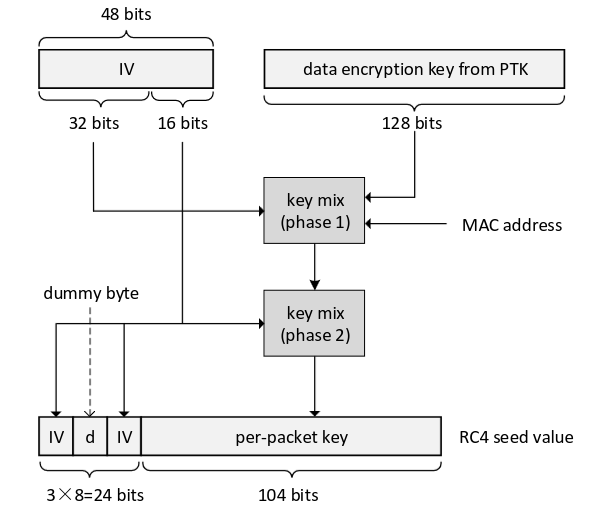
\includegraphics[width=0.5\textwidth]{img/wireless/TKIP key generation.png}
        \caption{TKIP generating RC4 keys}
      \end{figure}
      TKIP uses the same RC4 algorithm as WEP, but with a different key generation mechanism, but it 
      is still vulnerable to similar attacks, in particular to a MIC key recovery attack that, if 
      successfully executed, permits an attacker to transmit and decrypt arbitrary packets on the 
      network being attacked.\\
      The basis of the attack is an extension of the WEP chop-chop attack: because WEP uses a 
      cryptographically insecure checksum mechanism (CRC32), an attacker can guess individual
      bytes of a packet, and the wireless access point will confirm or deny whether or not the 
      guess is correct. If the guess is correct, the attacker will be able to detect the guess 
      is correct and continue to guess other bytes of the packet.\\
      However, with TKIP, the attacker must wait for at least 60 seconds after an incorrect guess 
      because if two incorrect Michael MIC codes are received within 60 seconds, the access point 
      will implement countermeasures, meaning it will rekey the TKIP session key, thus changing 
      future keystream.
    \end{subsubsection}
    
    \begin{subsubsection}{KRACK attack}
      The known weakness in WPA/TKIP is in the implementation of RC4, for this reason 
      WPA is not intended to be a long-term secure solution and users are recommended to 
      implement WPA2 whenever available.\\
      The only major weakness found in WPA2 is the Key Reinstallation Attacks (KRACK) targeting 
      the four-way handshake of the authentication protocol. In normal operation, when a client 
      joins a network and triggers the four-way handshake, a key is installed after receiving 
      message 3 for data confidentiality. However, if an attacker can intercept message 3 and
      replay it, the client will install the same key, but will increment the nonce, because Its
      tied to the packet number, and the replay counter used to prevent replay attacks.\\
      An attacker can force nonce resets by collecting and replaying message 3, and by doing so,
      he will ultimately be able to decrypt the packets.\\
      This kind of attacks can also be launched against group keys on WPA2.
      \begin{figure}[h]
        \centering
        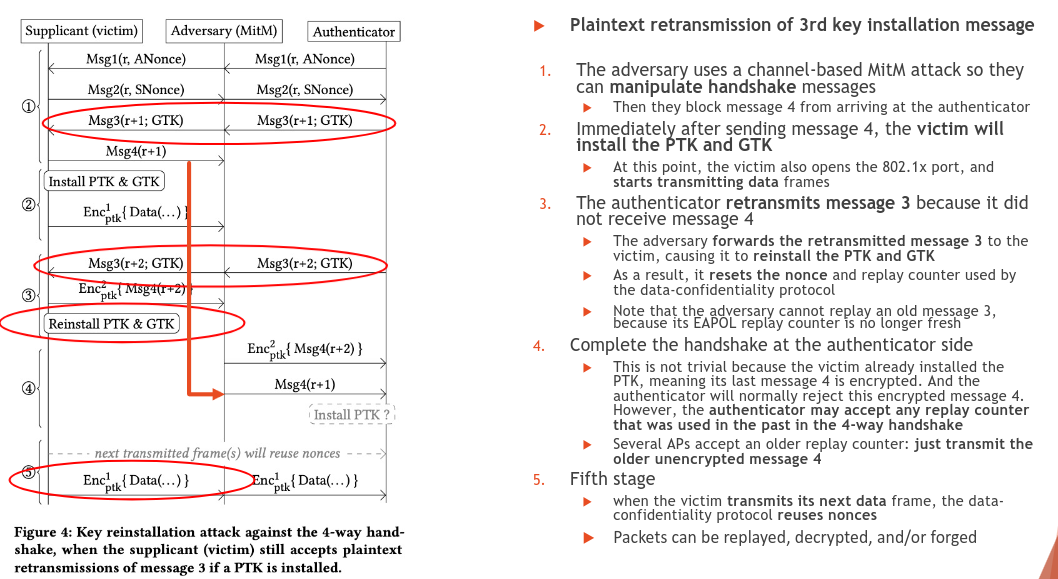
\includegraphics[width=0.9\textwidth]{img/wireless/KRAC attack.png}
        \caption{The KRACK attack}
      \end{figure}
    \end{subsubsection}

    \begin{subsubsection}{Opportunistic Wireless Encryption}
      OWE is a new standard that has been introduced in 2018, and is based on the Diffie-Hellman
      key exchange and HKDF(HMAC-based Extract-and-Expand Key Derivation Function) to enstablish
      the PKM that can be used for the encryption of the data. Its mainly used to protect open networks.
      The general idea is to generate the symmetric encryption key from the Elliptic Curve Diffie-Hellman
      key exchange, and then use the HKDF to derive the encryption key from the shared secret key 
      during the association phase. OWE supports both elliptic curve and finite field DH key exchange.

      \begin{figure}[h]
        \centering
        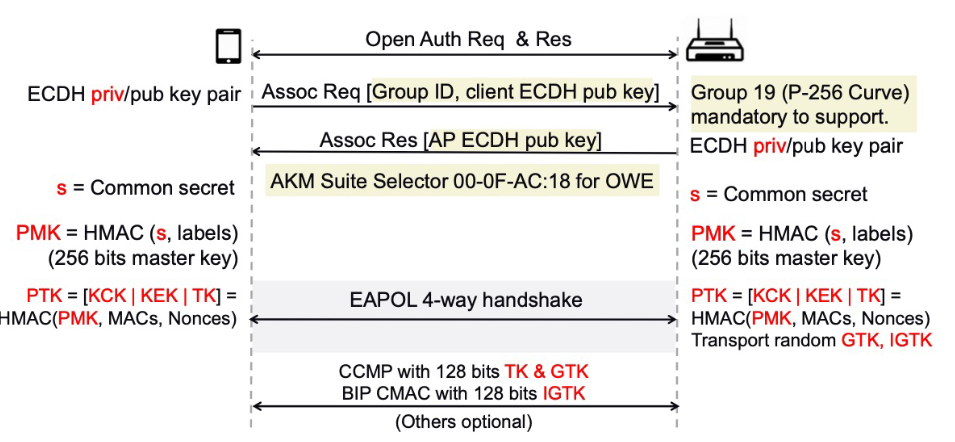
\includegraphics[width=0.5\textwidth]{img/wireless/owe.png}
        \caption{The OWE message exchange}
      \end{figure}

    \end{subsubsection}
    \begin{subsubsection}{Simultaneous Authentication of Equals}
      One of the major new features introduced in WPA3 is Simultaneous Authentication of Equals (SAE),
      which provides more robust password-based authentication, even when using a strong one, while 
      also providing protection against bruteforce attacks.\\
      SAE replaces the four-way handshake method (PSK) used in WPA2, thus being robust against 
      KRACK attack, because there's no need to know a PMK, but generates a PSK for the authentication
      process only, granting perfect forward secrecy, using ellictic curve DH too.\\
      \begin{figure}[h]
        \centering
        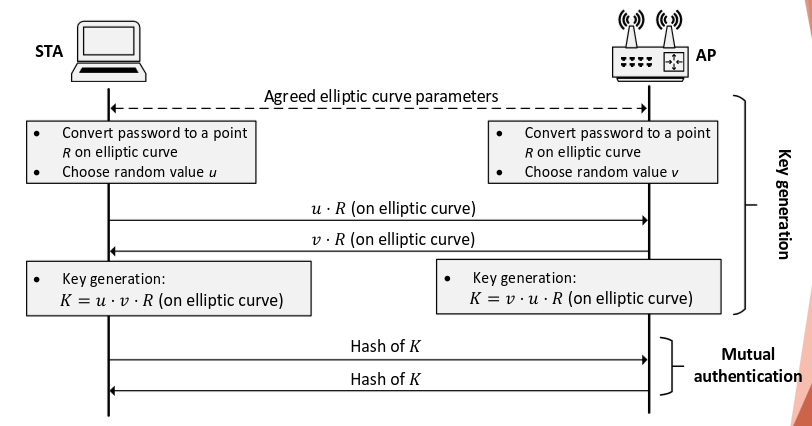
\includegraphics[width=0.5\textwidth]{img/wireless/sae.png}
        \caption{The SAE message exchange}
      \end{figure}
    \end{subsubsection}

  \end{subsection}

\end{section}

\begin{section}{Questions and answers}
  \begin{subsubsection}{What is the difference between the
    “infrastructure-based” and “ad-hoc” mode in a WLAN?}
    In infrastructure mode, all the traffic must pass trough the access point before reaching its
    destination, wheres in ad-hoc mode direct communication between nodes is possible(P2P).
  \end{subsubsection}
  \begin{subsubsection}{Why in infrastructure-based mode all traffic must go
      through the AP? What are the consequences in terms of performance in case
    two STA would like to exchange data?}
    There are a few reasons:
    \begin{itemize}
      \item to perform access control to the services of the network.
      \item to perform orchestration of the communications
      \item to kind of extend the range of the communications in some instances
    \end{itemize}
    This has a few drawbacks. In fact, if no direct communcations between nodes is possible, all
    traffic must pass trough the AP, which drasticaly reduce the trougput of data, because one
    packet pass trough two times. It makes also the communication more complex, which adds some
    overhead.
  \end{subsubsection}
  \begin{subsubsection}{How many independent channels are present in the 2.4GHz
    ISM IEEE 802.11 standard?}
    Over the 2.4GHz spectrum, 14 channels are available, but only 3 are indipendent.
  \end{subsubsection}
  \begin{subsubsection}{What are the maximum transmission rates for 802.11b?
    And for 802.11g? And for 802.11n?}
    For the 802.11b standard the MTR is 11Mbps, for 802.11g is 54Mbps, while for 802.11n is up to
    600Mbps.
  \end{subsubsection}
  \begin{subsubsection}{Describe the steps a STA has to follow to join a WLAN}
    To joind a WLAN, a STA has first to find an AP to connect to, either via probing requests or
    listening to beacon frames. To join the network and access its services it has to be both
    authenticated and associated. During the authentication process, the STA proves its identity to
    AP, and this is done either via open system authetication or a shared key trough a
    challenge-response authentication schema. During this process no confidentiality and integrity
    services are provided. Association is the next step, during which the STA and the selected AP
    exchanges the informations necessary to gain access to the network. If this step is successful,
    the STA joins the network, and is able to exchange data.
  \end{subsubsection}
  \begin{subsubsection}{What is the difference between Authentication and
      Association? Depict the sequence of frames observed when a STA
    successfully connects to a WLAN.}
    Authentication is the process of proving the identity of the STA to the AP or an authenticator
    in general, and is a step necessary to perform associaciation to an AP. association is the
    process of exchanging the necessary data to gain access to the network.
    Let's suppose that the station discovers an AP trough a probe request, the sequence of exchanged
    messages is: 
    \begin{itemize}
      \item Probe request 
      \item Probe response 
      \item Authentication request 
      \item Authetication response 
      \item Association request 
      \item Association response 
    \end{itemize}
  \end{subsubsection}
  \begin{subsubsection}{Describe the goals of the beacon frames. Which type of
    node can send such beacons?}
    Beacons are basically advertisement frames that an AP sends in broadcast to inform of its
    presence and the parameters necessary to connects to it, such as the SSID, the mac
    address,\dots The standard allows only the APs in infrastructure mode to send those
    periodically, which is an option set by default by the standard, but it can be disabled.
  \end{subsubsection}
  \begin{subsubsection}{Describe the goals of the probe frames. Which type of
    node can send such beacons?}
    Probes frames are messages sent by a STA in broadcast to discover which AP are in range. An AP
    which receives a probe request responds to it with a probe request with the informations
    necessary to connect to it, such as the SSID, the mac address, \dots Probe requests are sent by
    STAs, while probe requests are sent by the APs.
  \end{subsubsection}
  \begin{subsubsection}{What type of authentication mechanisms as supported by
    802.11?}
    The base version of 802.11 supports two authentication mechanisms:
    \begin{itemize}
      \item open system authentication: every autentication request is accepted
      \item shared key authentication, which is performed via challenge-response autentication 
    \end{itemize}
  \end{subsubsection}
  \begin{subsubsection}{Describe the problem of the hidden terminals. Provide
    some example to illustrate it.}
    The problem of the hidden terminal arises when two nodes connected to the same AP cant hear each
    other, but the signal is strong enough that two communications can collide at the AP, generating
    errors. This happens because the channel is half-duplex, so only one node can send and receive
    at the time, but because the two STAs cant hear ech other, they think that the channel is free,
    and can transmit data at the same time. This can be due to the distance between the two(fading)
    or an obstacle between them.
  \end{subsubsection}
  \begin{subsubsection}{Why a WLAN station cannot perform collision detection?
      What are the implications of this? Why in in 802.3 (ethernet) it is
    possible to detect collision instead?}
  \end{subsubsection}
  \begin{subsubsection}{Describe the CSMA/CA protocol in the case RTS/CTS are
    disabled}
    CMSA/CA, or carrier senses multiple access with collision avoidance, is a multiple access
    protocol for shared medium, which works as follows:
    \begin{enumerate}
      \item when a STA whant to transmit a packet, it listens to the channel, if its idle it tries
        to transmit after a short period of time(Distributed inter frame space, or DIFS). If the
        channel is sensed busy, it chooses a random binary exponential backoff value, which
        decreses while the channel is sensed free.
      \item when the counter reaches zero, the frame is transmitted when the channel is idle, and
        the STA waits for an ACK
      \item If the ACK is correctly received, alls good, otherwise it reenters the previous phase
        with another random counter with higher value. 
    \end{enumerate}
  \end{subsubsection}

  \begin{subsubsection}{Describe the CSMA/CA protocol in the case RTS/CTS are enabled.}
    If the RTS/CTS mechanism is implemented, a STA that wants to transmitt, if the channel is sent
    idle and the reservation time of a CTS message has expired, it can send a Request To Send
    message to the access point, which is basically a request to reserve the channel for a certain
    amount of time. The AP receives it, and proceeds to send in broadcast a Clear To Send message to
    all the connected STA in range, which signals the other STAs to non send anything for the
    specified time and allows the sender station to have exclusive access to the channel for the
    time being. The RTS request is sent after a DIFS while between all other packets elapses a SIFS.
  \end{subsubsection}
  \begin{subsubsection}{Depict the time-space plot in which station A sends to station B a data
    frame with the support of the AP in case RTS/CTS is enabled or is disabled.}
    See figure \ref{fig:rts-cts}.
  \end{subsubsection}
  \begin{subsubsection}{Does the probability of collision depend on the propagation time? Does the
    probability of collision depend on the transmission time? How?}
    With propagation time we refer to the time that a packet needs to reach the receiver while
    travelling a wireless channel. Of course it influences the probability of collision: if a packet
    takes too long to reach a certain node in the network, it could assume thaht the channel is idle
    and (assuming that no RTS/CTS mechanism is implemented and his EBT reaches zero and a DIFS has
    elapsed) try to transmit one of its messages, generating a collision.\\
    With transmission time we refer to the time needed to push the whole message on the channel. As
    delay is cumulative, it will also influence the probability of collision for the same reasons as
    before.
  \end{subsubsection}
  \begin{subsubsection}{Why does the receiver need to acknowledge the reception of a frame in
    CSMA/CA? What could happen if the receiver does not transmit the ACK?}
    In wireless links interface is high and the medium is not reliable at all, so a mechanism to
    ensure that the packet has correctly reached the destination is necessary. If its not
    implemented, a collision on a transmission could occur, and the packet would reach the
    destination damaged, without any way to notify to the sender that a collision has likely
    occurred.
  \end{subsubsection}
  \begin{subsubsection}{Why RTS/CTS can reduce the collision probability?}
    Having a reservation mechanism instead of multiple access detection one reduces drastically the
    probability of collision, because STA dont rely on a timer and to sense if the channel is idle,
    but will actually wait for the specified time to elapse. Still some collisions are possible, for
    example if two RST requests are sent at the same time, but are still much more unlikely.
  \end{subsubsection}
  \begin{subsubsection}{Why the control messages and the control part of a data frame must be
      transmitted at the minimum data rate? What could happen if those messages were transmitted at
    higher rates?}
    Control frames, or in general control data is used, as the name suggest, to handle changes or
    data that is important that reaches its destination. If this data would be transmitted at a
    higher data rate, the probability of error would also increase. Furthermore, an higher data rate
    implies a lower coverage of the signal, meaning that some STAs could receive a damaged message
    due to collisions, or not receive it at all. To sum it up, it for reliability and coverage
    reasons.
  \end{subsubsection}
  \begin{subsubsection}{Assume an AP would like to transmit a frame destined to all STAs in the WLAN
      (broadcast message). Depict the sequence of messages one would observe on the channel. At what
    rate would it be possible to transmit such a message? Which STA will send the ACK?}
    The AP, after detecting that the channel is idle, to avoid collisions, sends the packet with the
    broadcast address after a short preamble and waiting a DIFS. The transmission rate depends on
    the capabilities of each STA, as well as the AP, but it will be sent at the highest common data
    rate supported. The STAs that have received the packet correctly will then proceed to send back
    an ACKL packet at the basic data rate.
  \end{subsubsection}
  \begin{subsubsection}{In a 802.11 frames, how many MAC addresses are present? Why?}
    In a 802.11 frame, 4 address are present:
    \begin{itemize}
      \item the mac address of the sender
      \item the mac address of the receiver
      \item the mac address of the AP(or the source in general)
      \item mac address of the destination
    \end{itemize}
    The first two are obviously needed to indicate the two ends of the communication. The third one
    is needed because in infrastructure mode all the traffic must pass trough the AP, whilst the
    latter one is used in ad-hoc mode, being the mac destination address.
  \end{subsubsection}
  \begin{subsubsection}{Describe the 802.11 power management capabilities. How can a STA tell the AP
      it is going to sleep and for how long? How can the AP tell the STA that it has some buffered
    frames waiting to be sent?}
    In mobile devices power is a precious energy, for this reason 802.11 implements a power saving
    capabilities. A STA can notify the AP that its entering power saving mode by setting the
    power-management bit in the header of a frame, setting a timer to wake up just before receiving 
    a beacon frame from the AP. The STA will then enter the mode and the AP will start buffering the
    frames destined to it, instead of forwarding them. The beacon frame will contain a list of
    nodes with buffered frames, if no frame have as destination the STA, it re-enter PS mode,
    otherwise it can explicitly request the buffered frames via a polling message to the AP.
  \end{subsubsection}
  \begin{subsubsection}{Define the goodput and compute the maximum efficiency one could expect in an
    ethernet link where two nodes would like to exchange some traffic using UDP and IPv4.}
    The goodput is the ratio between the useful data at the application layer and the total length
    of the data received.\\
    UDP has an header length of 8 bytes, while IP has a 20 byte header and the ETH header is 38
    bytes long. The mtu of 1500 because of ETH. This means that the maximum efficiency is
    $\dfrac{1500-8-20}{1500+38}=95.71\%$
  \end{subsubsection}
  \begin{subsubsection}{Define the goodput and compute the maximum efficiency one could expect in an
    ethernet link where two nodes would like to exchange some traffic using TCP and IPv4.}
    As per the previous exercise, the overhead is 20B of TCP, 20B IPv4, meaning that the maximum
    efficiency is $\dfrac{1500-20-20}{1500+38}=94.93\%$
  \end{subsubsection}
  \begin{subsubsection}{Given the IPv4 header is 20 bytes long and the IPv6 header 40 bytes long,
    how would reduce the efficiency of a TCP file transfer in case the MTU is 1500 Bytes long?}
    As per previous exercise, $\dfrac{1500-20-40}{1500+38}=93.63\%$
  \end{subsubsection}
  \begin{subsubsection}{In the case of a half-duplex channel, why does the maximum goodput reduce?
    Provide an example.}
    In case of an half duplex channel, the goodput decreases, of course, due to awcknowledgments
    mainly. In fact, either a packet with useful data is transmitted, of an ACK is, and no other
    transmission is possible in the meanwhile. This means that the efficiency, in case of
    TCP+IP+ETH, becomes $\dfrac{1460}{(1500+38)+(38+20+20)}=90.34\%$.

  \end{subsubsection}
  % \begin{subsubsection}{The plot in the figure represents the efficiency of different IEEE 802.11
  %     versions versus the payload size (MSDU). Identify the maximum efficiency of a transmission in
  %     which the application at the sender side generates 1000 UDP messages of 500 bytes each.
  %   Consider an ideal scenario and a MTU of 1500 bytes.}
  % \end{subsubsection}
  \begin{subsubsection}{Consider a scenario in which a transmitter connected to an 802.11g (54Mb/s
      maximum rate) network sends a 200MB long file to a receiver connected to the AP using a
      100Mb/s ethernet link. What would be the maximum goodput one would expect? How long would it
    take to complete the file transfer?}
    Let's consider the bottomline efficiency of 802.11 to be 50\%, as explained during the lessions.
    Let's also assume that no packets are aggregated and the whole stack is using IPv4 and TCP, the
    efficiency for the wired portion of the link is 94.93\%. This means that the maximum achievable
    efficiency is $\text{min(94.93, 50)=50\%}$, while the goodput is $\text{min}(50\%\cdot
    54/2,94.93\%\cdot 100)=13.5Mbps$ as per the half duplex portion of the network. This means that to
    transfer the whole packet it would take $\dfrac{1600}{13.5}= \approx 119s$. 
  \end{subsubsection}
  \begin{subsubsection}{Consider a scenario in which a transmitter connected to an 802.11n (300Mb/s
      maximum rate) network sends a 200MB long file to a receiver connected to the AP using a
      100Mb/s ethernet link. What would be the maximum goodput one would expect? How long would it
    take to complete the file transfer?}
  \end{subsubsection}
  \begin{subsubsection}{Consider a scenario in which a transmitter connected to an 802.11n (300Mb/s
      maximum rate) network sends a 200MB long file to a receiver connected to the AP using a
      1000Mb/s ethernet link. What would be the maximum goodput one would expect? How long would it
    take to complete the file transfer?}
  \end{subsubsection}
  \begin{subsubsection}{Consider a scenario in which a transmitter connected to an 802.11n (300Mb/s
      maximum rate) network sends a 200MB long file to a receiver connected to the AP via the same
      802.11n technology. What would be the maximum goodput one would expect? How long would it take
    to complete the file transfer?}
  \end{subsubsection}
  
  \begin{subsubsection}{Describe possible denial of services attacks that leverage the 802.11
    authentication and association mechanisms. What type of messages would the attacker send? Which
  information will the attacker need to mount such an attack?}
    Authentication and association mechanisms of 802.11 can be exploited in a similar fashion, in
    fact, as there are association and authentication frames, there are also deauthentication and
    disassociation frames. This means means than an attacker can just send this kind of packets
    while spoofing the address of the victim to perform a denial of service attack, because the STA
    is unable to receive any data in this way, and have to either re-authenticate of associate
    itself with the AP again.
  \end{subsubsection}
  \begin{subsubsection}{Describe possible countermeasures to the de-authentication attacks.}
    A possible countermeasure against dAUTH attacks is based on the simple observation that users
    don't usually deauthenticate themselves and continue to send packets. An AP could just wait a
    small time interval before honouring a deAUTH request and keep listening if some packets keep
    coming from the same sender in the meanwhile. If no frame arrives, the request is honoured,
    otherwise it is dropped.\\ 
    Another countermeasure is based on the SNR, in fact an AP could measure the SNR level of a dAUTH
    request. If the legit traffic is used as a signature, if the request doesn't match it, it's just
    dropped.
  \end{subsubsection}
  \begin{subsubsection}{Describe possible DoS attacks that leverage weaknesses of the CSMA-CA
    mechanisms.}
    CMSA/CA tries to detect if the channel is busy to avoid collisions: if its sensed busy, so
    packet is send. A simple attack can exploit this schema by simply send enough packets so that
    the channel is sensed busy often enough that no legit node is sending any packet ever. If i
    recall correctly during the lectures it was stated that keeping the channel busy for one tenth
    of the channel capacity was enough to keep the channel "down".
  \end{subsubsection}
  \begin{subsubsection}{Describe a possible attack that leverages the NAVigation information
    provided in the 802.11 RTS/CTS mechanisms. Describe possible countermeasures to this attack.}
  \end{subsubsection}
    RTS/CTS mechanisms use 2 specia frames to reserve the channel for a given duration. Based on
    this observation, a simple attack could be mounted by simply sending a RTS request with the
    maximum length available(the reservation time field should be 16 bits long). By repeating this
    requests as the timer elapses, one can keep the channel busy indefinitely, disrupting any trial
    of legit communication, because no STA can transmit during the reserved period.\\
    This attack could be leveraged by simply limiting the time period for a reservation, to be big
    enough for legit communication.
  \begin{subsubsection}{Describe possible attacks that leverage the power-saving protocol of
    802.11.}
    A STA enters power saving mode by sending a frame with the power saving bit set to inform the AP
    that's "going to sleep". This will buffer the packets until it sends a request to forward them.
    An attacker can spoof a packet with the bit set to the AP, which will buffer the packets instead
    of sending them to the STA, effectively disrupting the communication. Another attack requires
    the spoofing of the AP, in fact it is possible to the STA that there are no packets for it,
    making it go to sleep.
  \end{subsubsection}
  \begin{subsubsection}{Why MAC authentication, IP filtering and SSID hiding are considered not
    valid mechanisms to protect a WLAN network?}
    Mac AUTH is useless because address can be spoofed, IP filtering is useless for the same reason
    and SSID hiding is useless because, even if beacons frames are suppresed, the SSID is still sent
    in clear in probe responses and association responses, which can be sniffed.
  \end{subsubsection}
  \begin{subsubsection}{Which are the security mechanisms WEP offers?}
    WEP offer confidentiality via encryption(RC4), integrity via a checksum(CRC32) and access
    control via shared password AUTH.
  \end{subsubsection}
  \begin{subsubsection}{Describe the shared key authentication mechanisms WEP supports. How can the
      AP verify the shared password? How is the shared password used to generate the stream cipher
    output?}
  \end{subsubsection}
  \begin{subsubsection}{Why is the shared key authentication deprecated?}
  \end{subsubsection}
\end{section}
